	\documentclass[a4paper,12pt]{article} 

\usepackage[unicode, pdftex]{hyperref}

% новая команда \RNumb для вывода римских цифр
\newcommand{\RNumb}[1]{\uppercase\expandafter{\romannumeral #1\relax}}

%Добавляет возможность искать и копировать текст
\usepackage{cmap}

%Убирает пробел между названием таблицы/рисунка и самой таблицей/рисунком
\usepackage{caption}
\captionsetup[table]{skip= -0 cm}
\captionsetup[figure]{skip= -0 cm}

%Выравнивание названия таблиц по левому краю
%\usepackage[nooneline]{caption} 
%Размеры отступов 
\usepackage[left=20mm, top=20mm, right=20mm, bottom=20mm, footskip=10mm]{geometry}

%Рисунки
\usepackage{graphicx}
\usepackage{wrapfig} %обтекание элементов
\graphicspath{{graphs}{figures}}  % папки с картинками

%Русский язык в формулах
\usepackage{mathtext}

%  Русский язык
\usepackage[T2A]{fontenc}			
\usepackage[utf8]{inputenc}			
\usepackage[english,russian]{babel}	

%Красная строка для первого абзаца
\usepackage{indentfirst}

%Готические буквы
\usepackage{amssymb}

% Математика
\usepackage{amsmath,amsfonts,amssymb,amsthm,mathtools} 
\usepackage{wasysym}

%Цветные подписи в таблице
\usepackage[table,xcdraw]{xcolor}

%Сделать несколько рядов одним
\usepackage{multirow}

\usepackage{fancyhdr} % Колонтитулы
 	\pagestyle{fancy}
 	\renewcommand{\headrulewidth}{0.3mm}  % Толщина линейки, отчеркивающей верхний колонтитул
 	%\lfoot{Нижний левый}
 	%\rfoot{Нижний правый}
 	\rhead{Белостоцкий Артмемий, Б04-006}
 	%\chead{Верхний в центре}
 	\lhead{Лабораторная работа №5.2.2}
 	\renewcommand{\footrulewidth}{0.3mm}
 	\cfoot{\thepage} % По умолчанию здесь номер страницы
 	
 	
%\captionsetup[table]{
%  position=above,
%  justification=raggedright,
  %labelsep=newline, % <<< label and text on different lines
%  singlelinecheck=false % <<< raggadright also when the cap%tion is shorter
                        % than a single line
%}
 	
\begin{document} 

%Титульник 
\begin{titlepage}
	\begin{center}
		\large 	МИНИСТЕРСТВО ОБРАЗОВАНИЯ И НАУКИ РОССИЙСКОЙ ФЕДЕРАЦИИ\\
				МОСКОВСКИЙ ФИЗИКО-ТЕХНИЧЕСКИЙ ИНСТИТУТ \\
				(НАЦИОНАЛЬНЫЙ ИССЛЕДОВАТЕЛЬСКИЙ УНИВЕРСИТЕТ)\\ 
				ФИЗТЕХ-ШКОЛА ЭЛЕКТРОНИКИ, ФОТОНИКИ \\
				И МОЛЕКУЛЯРНОЙ ФИЗИКИ \\
		
		
		\vspace{4.0 cm}
		Лабораторная работа № 5.2.2 \\ 
		\LARGE \textbf{Изучение спектров атома водорода \\ и молекулы йода}
	\end{center}
	\vspace{3 cm} \large
	
	\begin{flushright}
		выполнил студент 3 курса \\
		{группы Б04-006}\\
		\textbf{Белостоцкий Артемий}\\
	\end{flushright}
	
	\vfill

	\begin{center}
	Долгопрудный, 2022 г.
	\end{center}
\end{titlepage}                                                                      

\section*{Аннотация}

В данной работе будет вычислена постоянная Ридберга, путем исследования оптического спектра водорода. Также будет представлен анализ спектра поглощение паров йода в видимой области.

\section*{Теоретические сведения}

\subsubsection*{Спектр атома водорода}

Атом водорода является простейшей атомной системой, для которой уравнение Шредингера (\ref{eq1:Shredinger}) может быть решено точно. 

\begin{align} \label{eq1:Shredinger}
	-\frac{\hbar^2}{2m} \Delta \psi - \frac{e^2}{r} \psi = E \psi
\end{align}

Именно поэтому спектр атома водорода является предметом тщательного экспериментального исследования. Длины волн спектральных линий атома водорода описываются формулой:

\begin{align}
	\frac{hc}{\lambda_{nm}} = R \left( \frac{1}{n^2} - \frac{1}{m^2} \right),
\end{align}

где $R$ -- константа, называемая постоянной Ридберга, а $m, n$ -- целые числа.

\begin{figure}[h!]
	\centering
	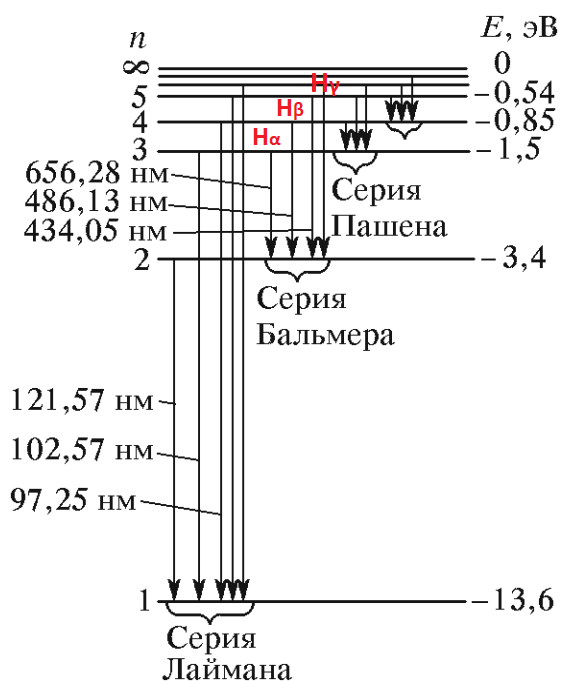
\includegraphics[width=0.6\linewidth]{Hydrogen_spectre}
	\caption{Спектр атомарного водорода}
\end{figure}


В данной работе будут наблюдаться 3 линии из серии Бальмера (n = 2), а именно -- $H_{\alpha}, H_{\beta}, H_{\gamma}$

\pagebreak

\subsubsection*{Спектр молекулы йода}

Молекулы обладают более богатым спектром возбужденных состояний, чем изолированные атомы, в молекулах могут возбуждаться дополнительные степени свободы: колебания составляющих их атомов друг относительно друга и вращения молекул относительно различных осей. Энергии вращательных и колебательных уровней задаются выражениями:

\begin{align*}
	E_{вращ} = \frac{\hbar^2}{2J} l(l+1), 
\end{align*}

где $J$ -- момент инерции молекулы относительно оси вращения, $l = 0, 1, 2, \dots$

\begin{align*}
	E_{колеб} = \hbar \omega_0 \left( n + \frac{1}{2} \right),
\end{align*}

где $\omega_0$ -- собственная частота осциллятора, $n = 0, 1, 2, \dots$

Также приведем отношение характерных энергий вращательного и колебательного возбуждения:

\begin{align*}
	\frac{E_{колеб}}{E_{вращ}} \approx \frac{1}{\sqrt{\frac{m_e}{M_{яд}}}} \approx 10^3
\end{align*}

Именно поэтому вращательные степени свободы в данной лабораторной работе видны не будут.

\begin{figure}[h!]
	\centering
	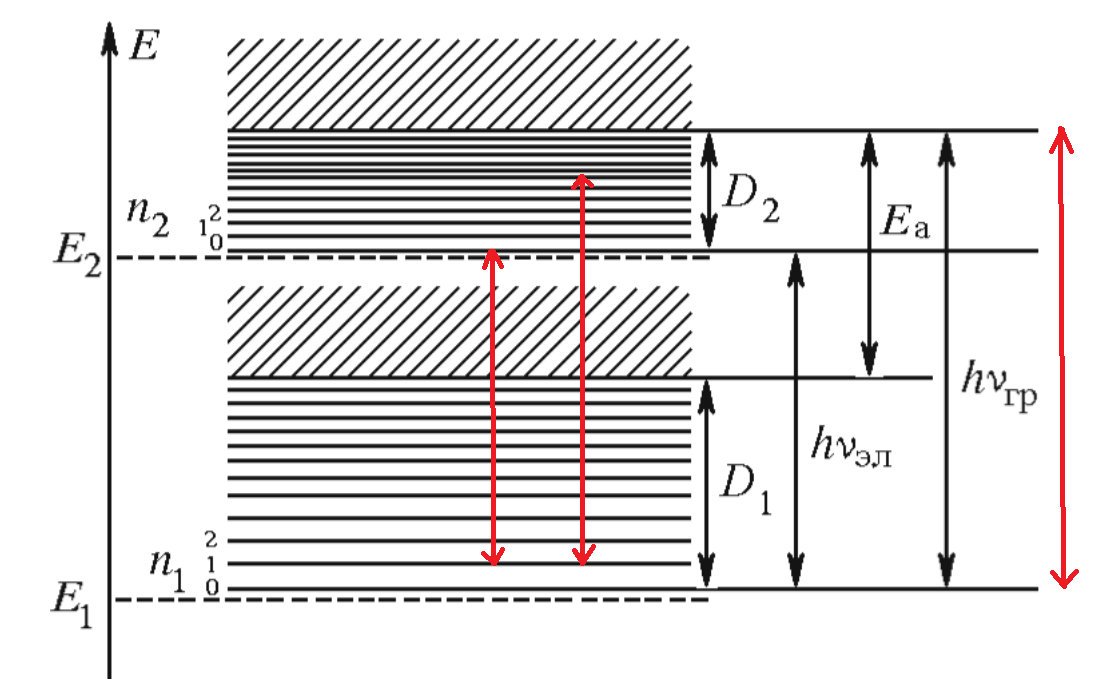
\includegraphics[width=0.8\linewidth]{Oscillating_levels}
	\caption{Электронные и электронно-колебательные энергетические уровни молекулы йода. Красным отмечены переходы, которые наблюдались в работе (взято из описания лабораторной работы)}
	\label{fig1:osc_lvl}
\end{figure}


\pagebreak

\subsection*{Экспериментальная установка}

\begin{figure} [h!]
	\centering
	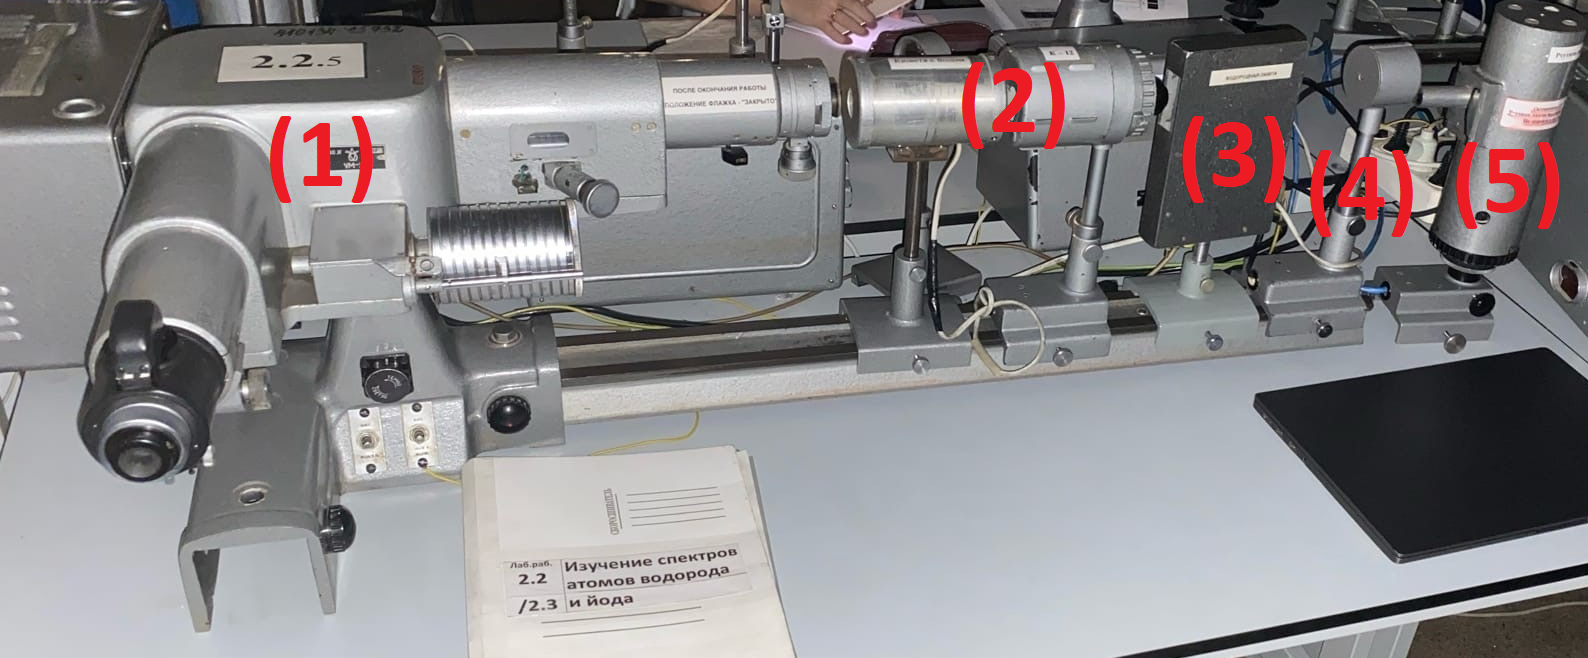
\includegraphics[width=\linewidth]{setup}
	\caption{Экспериментальная установка. (1) -- монохроматор, (2) -- кювета с йодом и лампа накаливания, (3) -- водородная лампа, (4) -- неоновая лампа,(5) -- ртутная лампа}
\end{figure}

\subsection*{Ход работы}

Используя окуляр и неоновую лампу, проградуируем барабан монохроматора, зная спектр неоновой лампы.

\begin{figure}[h!]
	\centering
	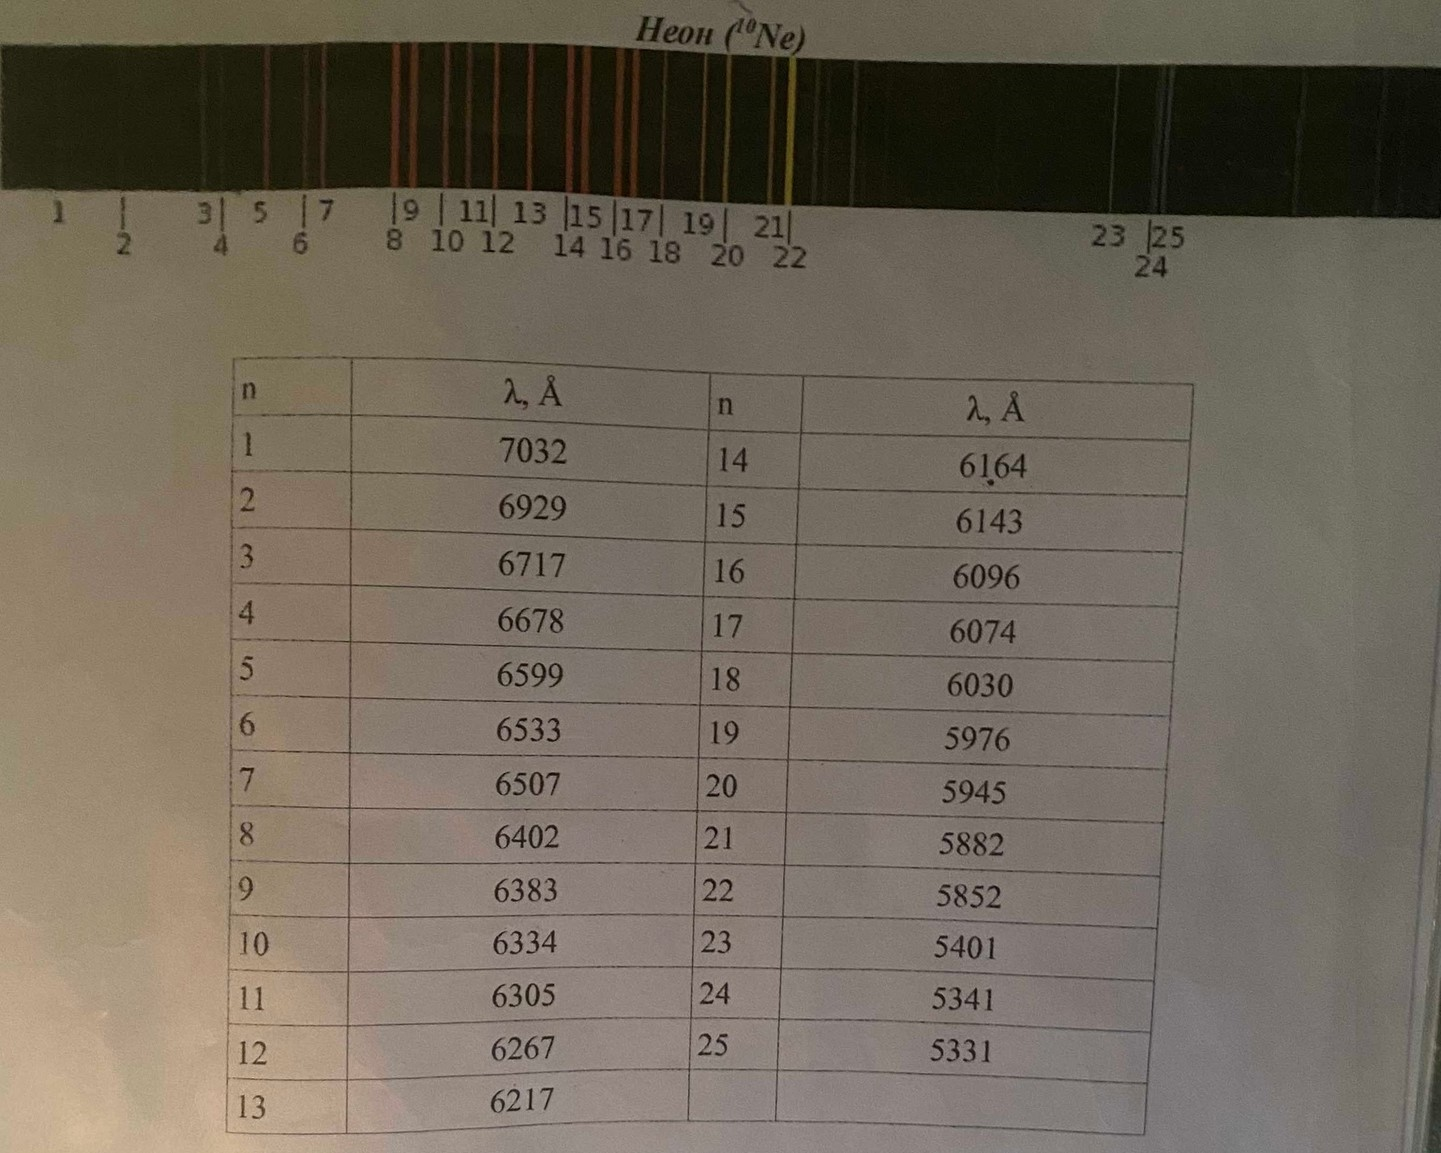
\includegraphics[width=0.8\linewidth]{theor_neon_spectre}
	\caption{Спектральные линии неона и соответствующие им длины волн}
\end{figure}

\pagebreak

\begin{figure}[h!]
	\centering
	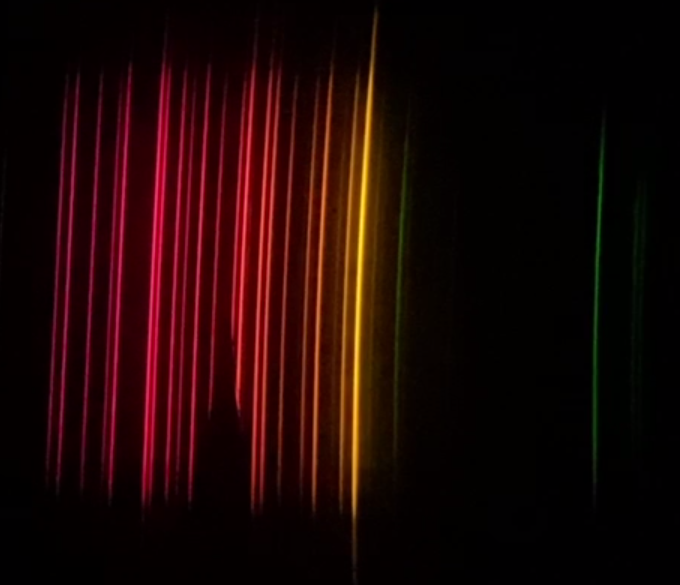
\includegraphics[width=0.7\linewidth]{neon_spectre}
	\caption{Спектральные линии неона, полученные экспериментально}
\end{figure}

Аналогично проградуируем спектрометр по спектру ртути.

\begin{figure}[h!]
	\centering
	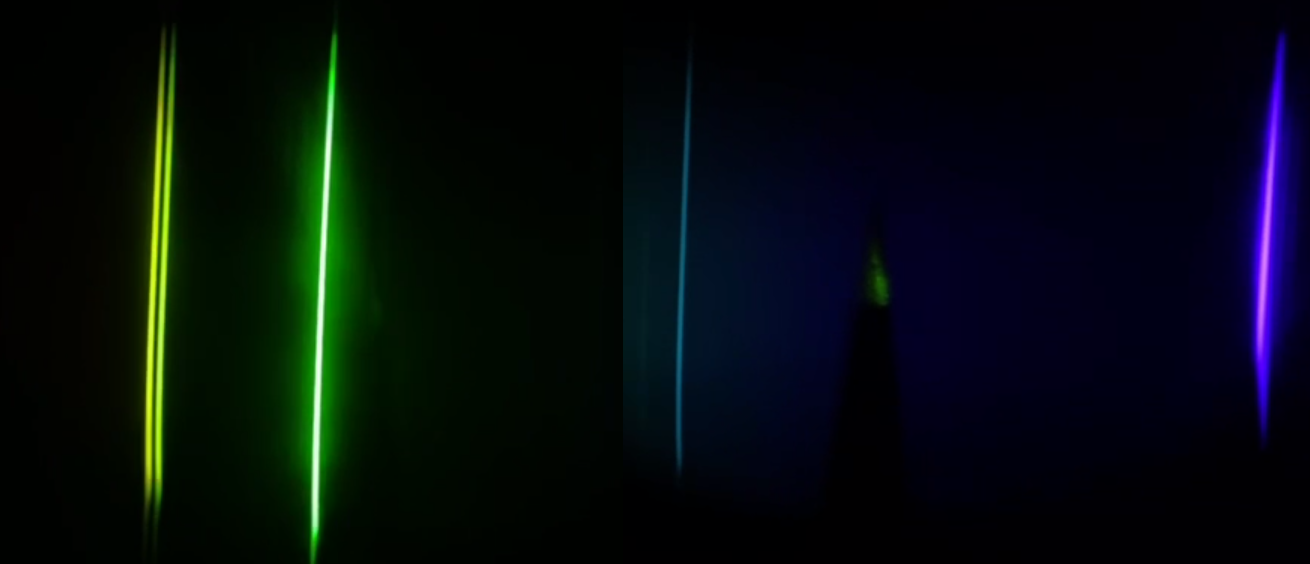
\includegraphics[width=\linewidth]{Hg_spectre}
	\caption{Экспериментальный спектр линий паров ртути}
\end{figure}	

\pagebreak
	
\begin{figure}[h!]
	\centering
	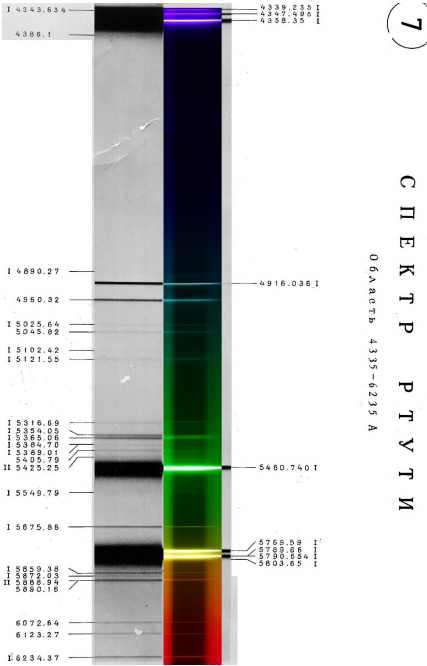
\includegraphics[width=0.7\linewidth]{theor_Hg_spectre}
	\caption{Спектр линий паров ртути в видимом диапазоне. (взято из описания лабораторной работы)}
\end{figure}

По полученным данным построим график зависимости угла, указываемого на барабане, от длины волны спектральных линий $Ne$ и $Hg$

Аппроксимируем калибровочную кривую полиномом степени $n$, учитывая что мы хотим получить минимум погрешности коэффициентов и не большое количество самих коэффициентов (т.к. погрешности будут складываться). Анализируя разные $n$ (графики представлены в Приложении), остановим свой выбор на $n = 3$

\pagebreak

\begin{figure}[h!]
	\centering
	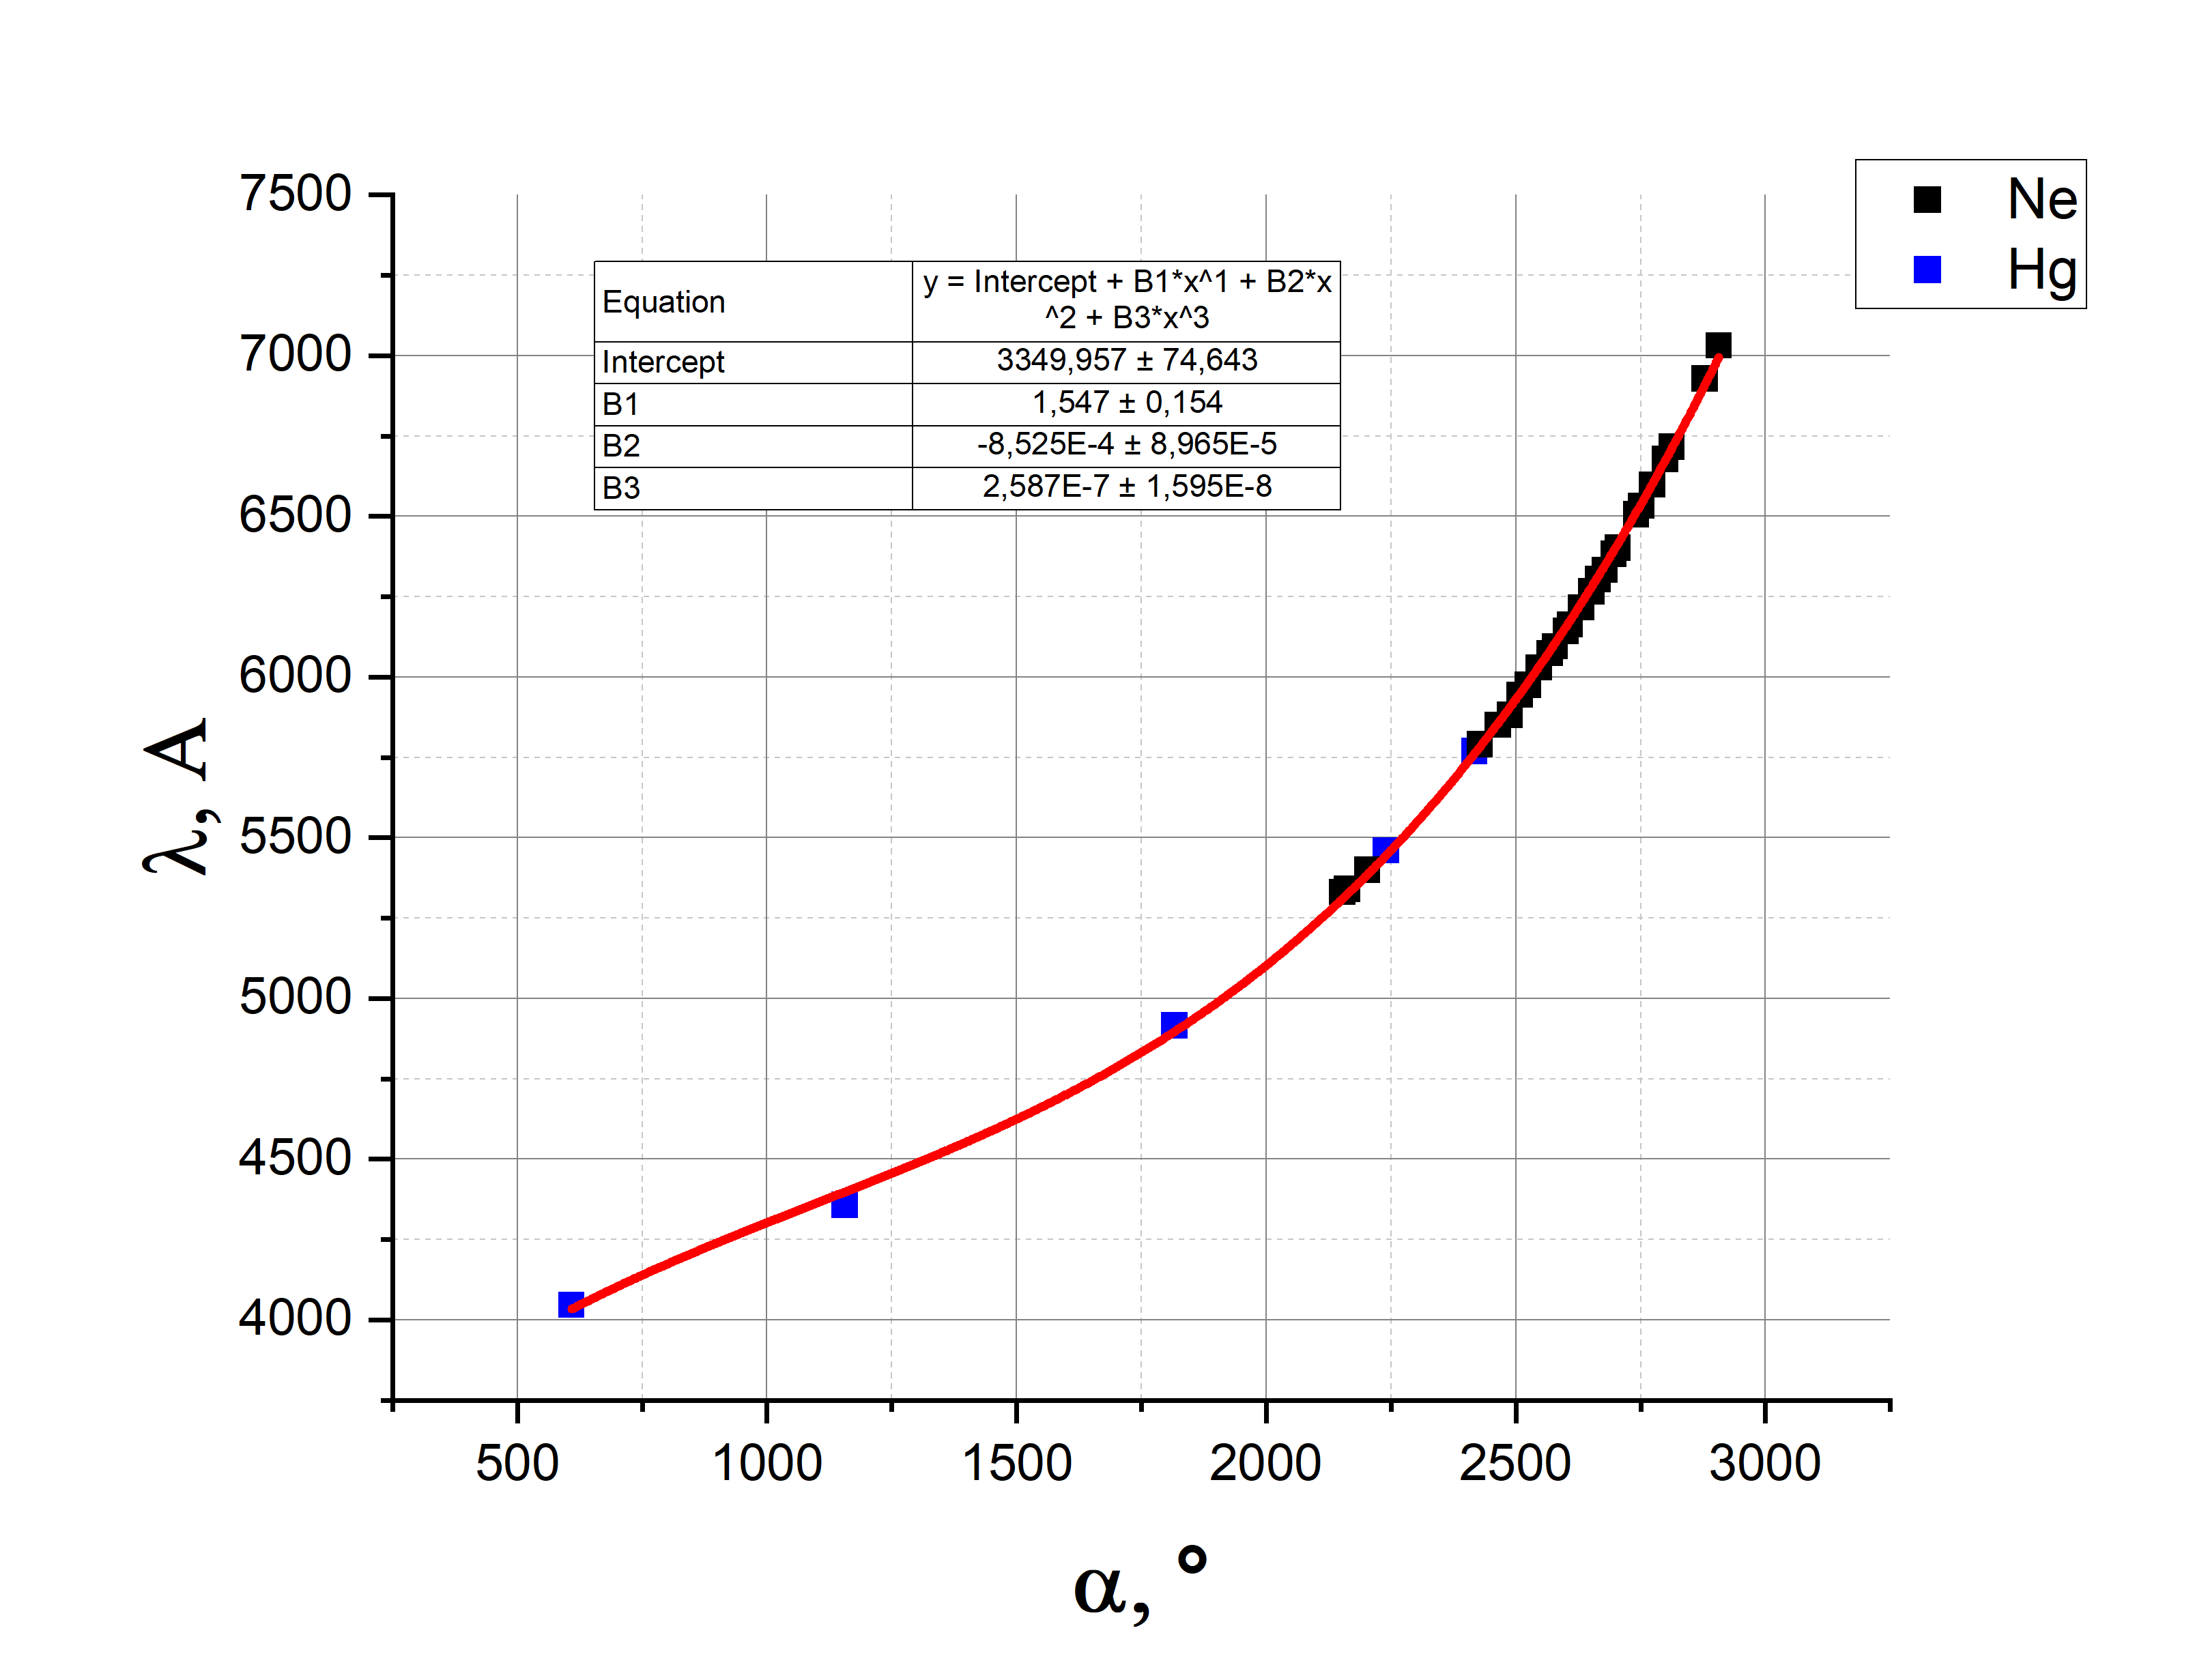
\includegraphics[width=\linewidth]{Calibration (3 degree polynom)}
	\caption{Калибровочный график зависимости угла, указанного на барабане монохроматора от длины волны спектральной линии $Ne$ и $Hg$}
\end{figure}

\subsubsection*{Спектр водорода}

Снимем спектр водорода. Измерим положение линий $H_{\alpha}, H_{\beta}, H_{\gamma}$. Полученные данные занесем в Таблицу \ref{table1:hydrogen}

\begin{figure}[h!]
	\centering
	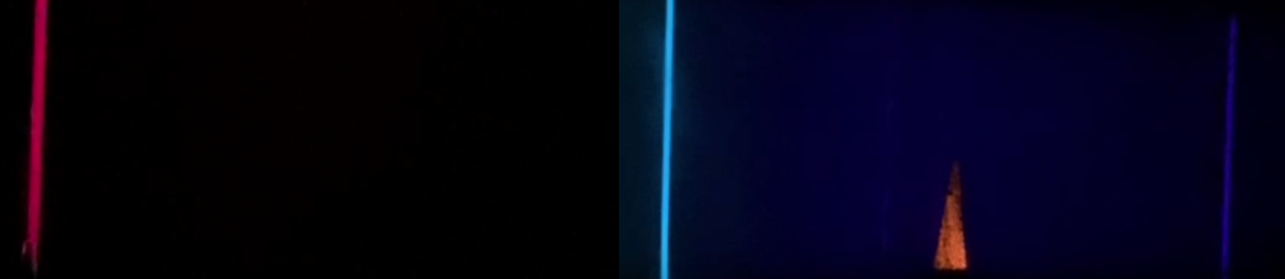
\includegraphics[width=\linewidth]{Hydrogen_spectre_2}
	\caption{Экспериментальный спектр водорода}
\end{figure}	

\begin{table}[h!]
	\centering
	\caption{Полученные длины волн спектра водорода}
	\label{table1:hydrogen}
	\begin{tabular}{|c|c|c|}
	\hline
	Линия & $\alpha, \circ$ & $\lambda$, нм \\ \hline
	$H_{\alpha}$ & 1132 & 438,6 \\ \hline
	$H_{\beta}$ & 1768 & 485,4 \\ \hline
	$H_{\gamma}$ & 2762 & 657,5 \\ \hline
	\end{tabular}
\end{table}

\pagebreak

С помощью калибровочного графика определим длины волн линий $H_{\alpha}, H_{\beta}, H_{\gamma}$. Построим график зависимости $\frac{1}{\lambda}$ от  $\left( \frac{1}{4} - \frac{1}{m^2} \right)$, по наклону графика определим константу Ридберга.

\begin{figure}[h!]
	\centering
	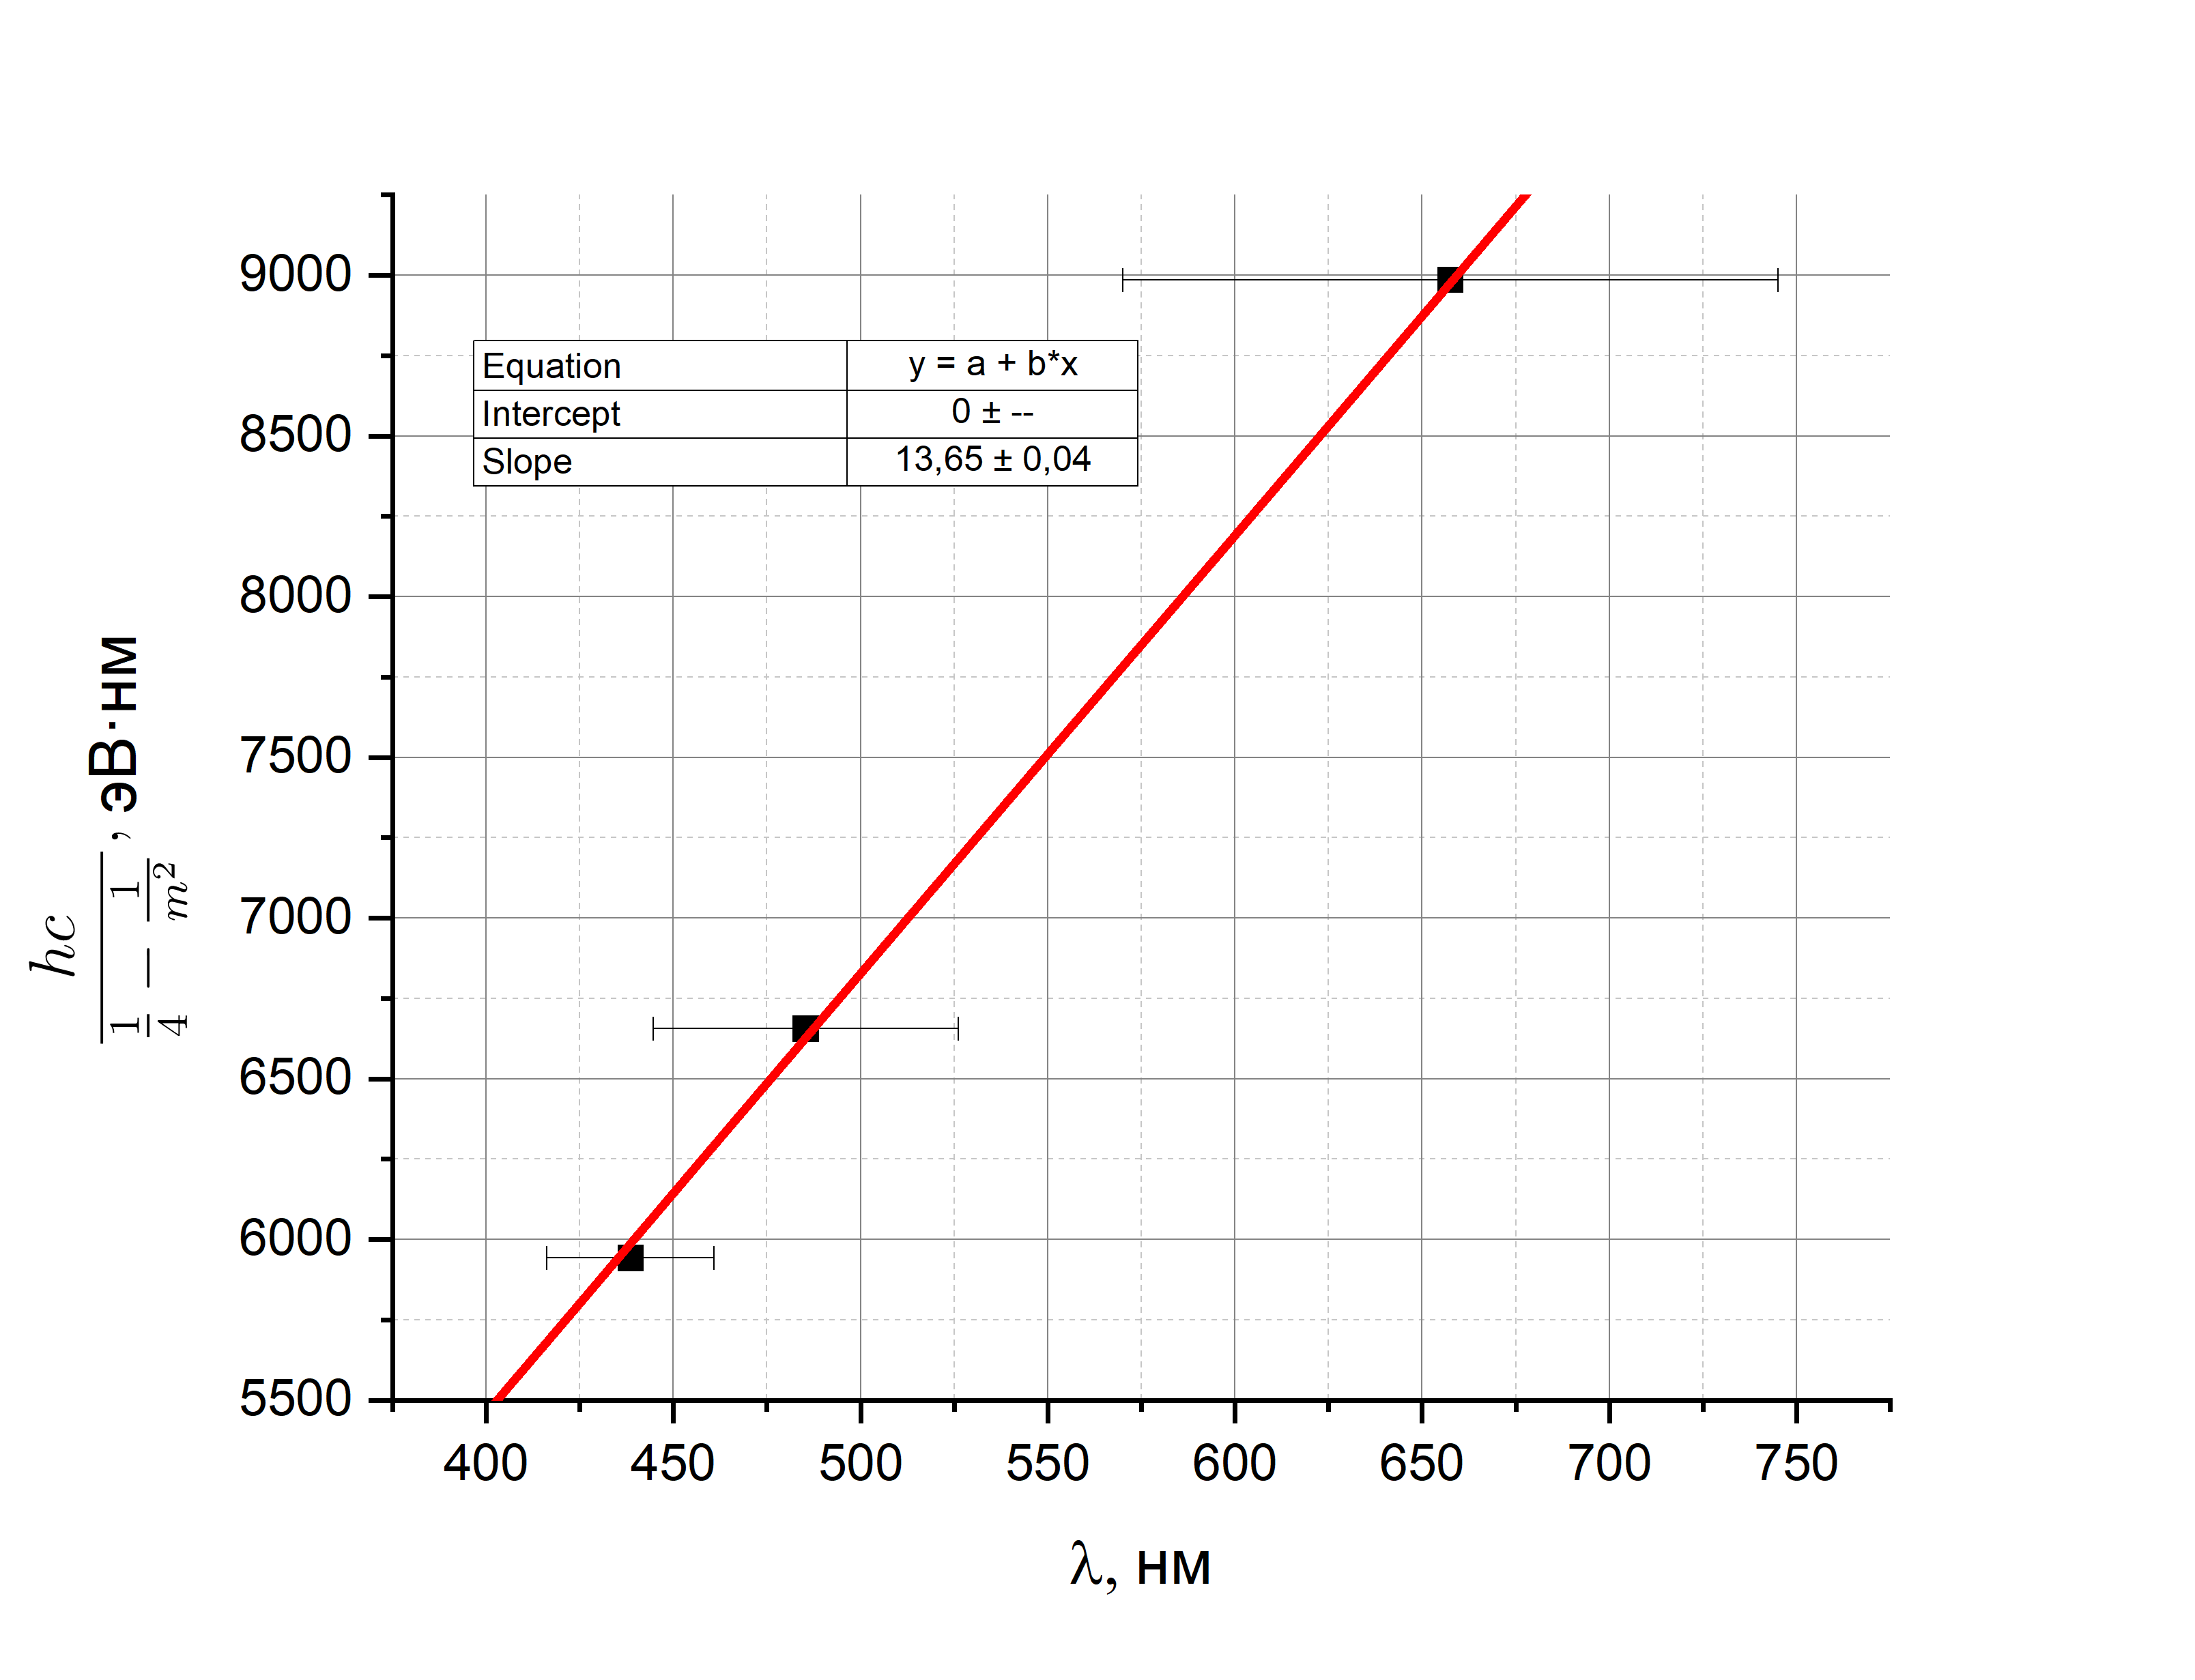
\includegraphics[width=\linewidth]{Hydrogen}
	\caption{График зависимости $\lambda = f \left(\frac{hc}{\frac{1}{4} - \frac{1}{m^2}} \right)$}
\end{figure}	

Из графика получаем:

$$
	R \approx 13,65 \pm 0,04 \ эВ
$$

\newpage

\subsubsection*{Спектр йода}

Получим спектр поглощения йода.

Измерим положения 3 полос поглощения: самой левой, шестой по счету от крайней левой и крайнюю правую. Полученные данные занесем в Таблицу \ref{table2:iodium}

\begin{figure}[h!]
	\centering
	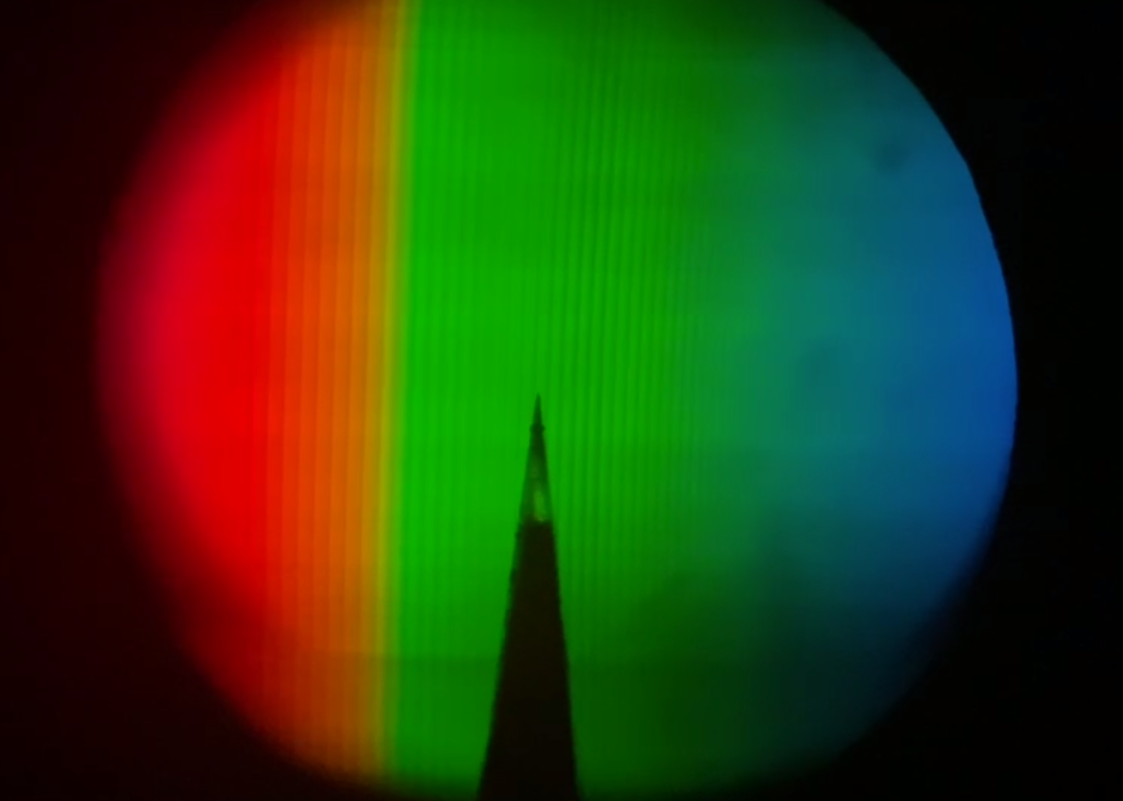
\includegraphics[width=\linewidth]{Iodin_spectre}
	\caption{Экспериментальный спектр поглощения йода (темные полосы)}
\end{figure}	

\begin{table}[h!]
	\centering
	\caption{Полученные длины волн для спектра поглощения йода}
	\label{table2:iodium}
	\begin{tabular}{|c|c|c|}
	\hline
	Линия & $\alpha, \circ$ & $\lambda$, нм \\ \hline
	Крайняя левая & 2624 & 621,8 \\ \hline
	Шестая от крайней левой & 2516 & 597\\ \hline
	Крайняя правая & 2038 & 515,6 \\ \hline
	\end{tabular}
\end{table}

Вычислим энергию колебательного кванта возбужденного состояния молекулы йода:

$$
	h \nu_2 = (h\nu_{1,5} - h \nu_{1,0})/5 \approx 17 \ мэВ
$$

Оценим энергию электронного перехода $h\nu_{эл}$ (см. Рис.\ref{fig1:osc_lvl}), зная что энергия нулевых колебаний основного состояния равна $h \nu_1 = 0,027 $ эВ.

$$
	h\nu_{эл} = h \nu_{1,0} + h\nu_1 \approx 2,03 \ эВ
$$

Оценим энергию диссоциации молекулы в основном состоянии $D_1$ (см. Рис.\ref{fig1:osc_lvl}), измерив величину $h\nu_{гр}$ и зная $E_a$:

$$
	D_1 = h\nu_{гр} - E_a = (2,41 - 0,94) эВ = 1,47 \ эВ
$$

Оценим энергию диссоциации молекулы в возбужденном состоянии:

$$
	D_2 = h\nu_{гр} -  h\nu_{эл} = (2,41 - 2,03) эВ = 0,38 \ эВ
$$

\section*{Обсуждение результатов}

\subsubsection*{Сравнение кванта колебательной энергии и температуры}

При средней комнатной температуре $T = 298 \ К, \ kT \approx 0,026 \ эВ$, расстояние между колебательными уровнями энергии основного состояния $\Delta E = 0,027 \ эВ \sim kT$, а энергия электронного перехода $h\nu_{эл} \gg kT$. 

Таким образом, можем предположить, что колебательные уровни основного состояния заселены, а колебательные уровни возбужденного состояния почти не заселены.

Оценим вклад колебательных степеней в теплоемкость молекулы йода. Из курса термодинамики (а именно, из задач домашнего задания) мы знаем, что, используя статистические методы, возможно рассчитать теплоемкость, которую <<создают>> только колебательные степени свободы:

$$
	c_v = \frac{\partial <\varepsilon>}{\partial T} \cdot N_A = \left(\frac{h\nu}{kT}\right)^2 \frac{e^{\frac{h\nu}{kT}}}{(e^{\frac{h\nu}{kT}} - 1)^2} \approx 0.91 R
$$

Тогда, учитывая что молекула имеет 3 поступательные степени свободы и 2 вращательные, полная теплоемкость паров йода:

$$
	c_V = \frac{5}{2} R + 0.91 R = 3.41 R = 28,3 \frac{Дж}{К \cdot моль}
$$

\section*{Выводы}

\begin{itemize}
	\item В ходе работы была вычислена постоянная Ридберга $R = 13,65 \pm 0,04 \ эВ$, что, в пределах погрешности, совпадает с табличным результатом $R = 13,61 \ эВ$
	\item Были оценены энергии диссоциации молекулы йода в основном $D_1 = 1,47 \ эВ$ и возбужденном состоянии $D_2 = 0,38 \ эВ$
	\item Также была оценена теплоемкость паров  йода $c_V \approx 20,1 \frac{Дж}{К \cdot моль} $
\end{itemize}



\end{document}